\chapter{RESULTS AND DISCUSSIONS}
\label{chap:result}

\section{Experiments}
We thoroughly investigate our proposed algorithms on synthetic as well as real datasets and conduct extensive experiments through systematic evaluation. We use $k$-means algorithm as baseline for number of components identification (see Algorithm~\ref{alg:k-comp-id}) from data (NOT graph!). Whereas, it is not possible to compare the performance of bipartite identification (see Algorithm~\ref{alg:bip-id}) for real datasets, we demonstrate its performance for synthetic dataset.
\paragraph{Synthetic datasets} We first construct an adjacency matrix for multi-component graph and bipartite graphs such that the laplacian matrix is positive semi-definite i.e. $\mathbf{\Theta}^{\dagger} \succeq 0$. The edge weights are considered equal for simplicity. This is the true precision matrix of the graph. We compute the pseudo-inverse of precision matrix to get the covariance matrix. We sample $n$ observations from the $p$-dimensional multivariate normal distribution $\mathbf{X} \sim \mathcal{N}\left(0, \Theta^{\dagger}\right)$ to obtain the synthetic data. We open source all our codes and experiments to further advance the research in graph learning and graph model selection on \href{https://github.com/anshul3899/Structured-Graph-Learning}{Github}.

\paragraph{Real datasets}
We empirically evaluate the performance of our algorithms on following multivariate real datasets:
\begin{enumerate}
	\setlength\itemsep{0.5em}
	\item \textbf{Cancer RNA-Seq dataset} We consider the huge dataset \citep{weinstein2013cancer} consisting of 801 nodes and 20531 samples. It consists of genetic features of patients having 5 types of cancers: breast carcinoma (BRCA), kidney renal clear-cell carcinoma (KIRC), lung adenocarcinoma (LUAD), colon adenocarcinoma (COAD), and prostate adenocarcinoma (PRAD). Due to computational limitations, we consider a subset of the data consisting of first 70 nodes following \cite{kumar2020unified}.
%	\item \textbf{Abalone dataset} The goal is to predict the age of the abalone fish \citep{nash1994population}. Instead of prediction, age is converted into 29 classes. The attributes are dimensions and different organ weights of the fish. The dataset comprises of 1477 samples and 8 attributes. 
%	\item \textbf{Yeast dataset} The goal is to predict localization sites of proteins: CYT, NUC, MIT, ME3, ME2, ME1, EXC, VAC, POX, ERL. The dataset \citep{nakai1991expert} consists of 1484 samples of 9 attributes
	\item \textbf{Iris dataset} It consists of sepal and petal dimensions of 3 different species of iris flowers: Iris Setosa, Iris Versicolour and Iris Virginica. The dataset \citep{fisher1936use} comprises of 150 samples with 4 feature attributes.
%	\item \textbf{Animals dataset} The dataset \citep{smith1993similarity} consists of answers to 102 categorical questions for 33 animals based on similarity among them.
\end{enumerate}

Both the above datasets are available at UCI Machine Learning Repository.

\subsection{Evaluation metrics}
We use the Relative Error and F1-score metrics for evaluation of synthetic datasets where both the true precision matrix $\Theta^{\dagger}$ is known. $\hat{\Theta}$ is the estimated precision matrix through our algorithms. In case of real datasets, we use accuracy for the number of components identified in the data and visual inspection for the animals dataset where we don't know the true number of components. In F1-score, True Positive (tp) denotes the case when there is an edge in the actual graph and the estimated graph also predicts an edge; False Positive (fp) stands for the case when there is no edge in true graph but there is an edge in the estimated graph; and false negative (fn) denotes the case when there is an edge in the true graph but the estimated graph misses it. F1-score takes values between 0 and 1 where 1 denotes perfect structure recovery \citep{egilmez2016graph}.
$$
\mathbf{\text { Relative Error }=\frac{\left\|\hat{\Theta}-\Theta^{\dagger}\right\|_{F}}{\left\|\Theta^{\dagger}\right\|_{F}}, \text { F1-Score }=\frac{2 \operatorname{tp}}{2 \operatorname{tp}+\mathrm{fp}+\mathrm{fn}}}
$$

\section{Results}

We present the results for Algorithm~\ref{alg:k-comp-id} and Algorithm~\ref{alg:bip-id} in this section.
\subsection{Component identification}

\subsubsection{Synthetic Datasets}

\textbf{Data generation:} samples $\mathbf{X}=\left\{\mathbf{x}^{(i)} \in \mathbb{R}^{p}\right\}_{i=1}^{n}$ from a 4-component GGM with 10 nodes in each component such that $n=1200$ and $p=40$, assuming equal number of nodes in each component and equal edge weights.

We test our proposed Algorithm~\ref{alg:k-comp-id} on the above data by feeding in the sample covariance matrix $S$ to SGL algorithm for different number of components $k$. The learned $k$-component graphs are shown in Fig~\ref{fig:kcomp-adj}, where we can clearly see the learned graph for $k=4$ is most likely to be the true graph which can be also be visually confirmed. Our algorithm predicts the number of components in the graph from which the data is sampled is $4$ as it has obtained the maximum eBIC score in Fig~\ref{fig:kcomp-ebic}. Infact, our algorithm is not only accurately able to infer the true number of components from the data, but also able to clearly distinguish between bipartite and multi-component graph. Bipartite graph structure earns eBIC score of $789.834$ which is much lower than the eBIC score of 4-component graph structure, thus distinguishing between the two. F1-scores, relative error and eBIC scores for all graph structures can be seen in Table~\ref{tab:kcomp-res}.

%TODO: Uncomment below code
\begin{figure}[htpb]
	\begin{subfigure}{\linewidth}
		\includegraphics[width=.3\linewidth]{kcomp_true_adj_ktrue=4}\hfill
		\includegraphics[width=.3\linewidth]{kcomp_estimated_adj_empirical}\hfill
		\includegraphics[width=.3\linewidth]{kcomp_estimated_adj_k=1}
		\caption{}
	\end{subfigure}\par\medskip
		\begin{subfigure}{\linewidth}
		\includegraphics[width=.3\linewidth]{kcomp_estimated_adj_k=2}\hfill
		\includegraphics[width=.3\linewidth]{kcomp_estimated_adj_k=3}\hfill
		\includegraphics[width=.3\linewidth]{kcomp_estimated_adj_k=4}
		\caption{}
	\end{subfigure}\par\medskip
		\begin{subfigure}{\linewidth}
		\includegraphics[width=.3\linewidth]{kcomp_estimated_adj_k=5}\hfill
		\includegraphics[width=.3\linewidth]{kcomp_estimated_adj_k=6}\hfill
		\includegraphics[width=.3\linewidth]{kcomp_estimated_adj_k=7}
		\caption{}
	\end{subfigure}\par\medskip
	\begin{subfigure}{\linewidth}
	\includegraphics[width=.3\linewidth]{kcomp_estimated_adj_k=8}\hfill
	\includegraphics[width=.3\linewidth]{kcomp_estimated_adj_k=9}\hfill
	\includegraphics[width=.3\linewidth]{kcomp_estimated_adj_k=10}
	\caption{}
	\end{subfigure}\par\medskip
	\caption{True, empirical and estimated adjacency matrix for $k=1,2,...,10$ component graphs}
	\label{fig:kcomp-adj}
\end{figure}

\begin{center}
	\begin{figure}[htpb]
		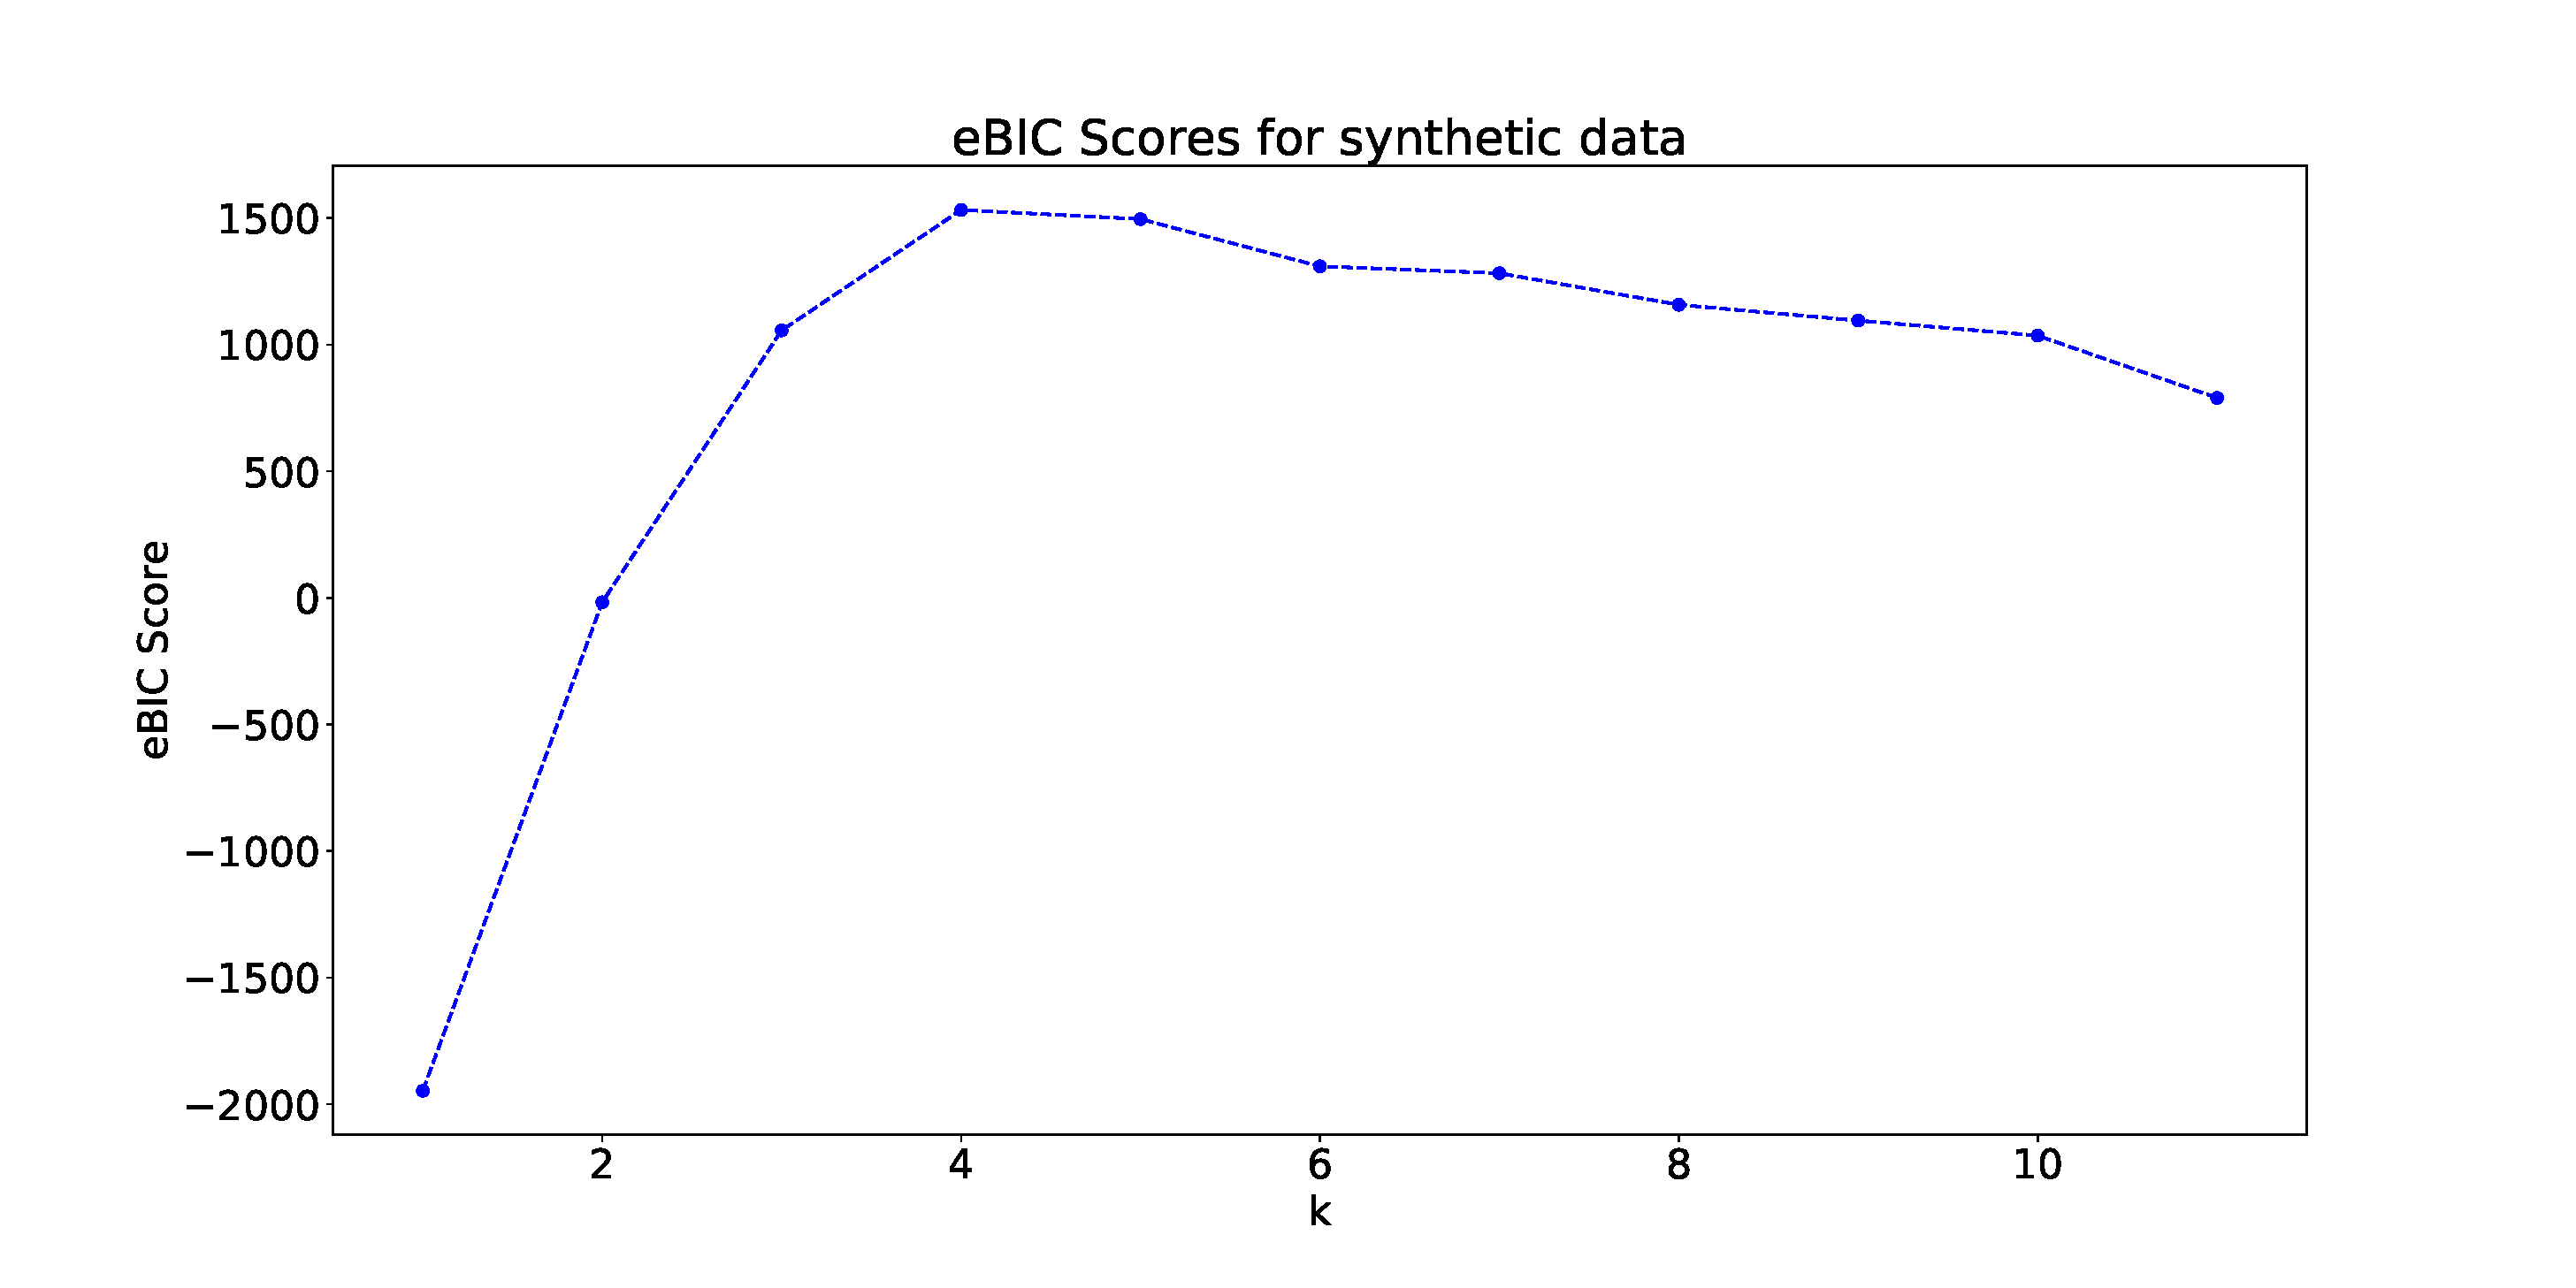
\includegraphics[scale=0.32]{Pictures/4comp}
		\caption{Plot of eBIC scores for 4-component GGM synthetic data}
		\label{fig:kcomp-ebic}
	\end{figure}
\end{center}

\begin{table}[htpb]
	\caption{k-component graph structure identification results on 4-component GGM}
	\label{tab:kcomp-res}
	\centering
	\begin{tabular}{llll}
		\toprule
		Metric     &   F1-Score  & Relative Error & eBIC Score \\
		\midrule
		
		
		True Adj          & 1.000  & 0     &    \\
		Empirical Adj     & 0.375  & 0.375 &    \\
		1-component Adj   & 0.375  & 0.341 &  $-$1946.963	 \\
		2-component Adj   & 0.534  & 0.678 &  $-$17.131  \\
		3-component Adj   & 0.728  & 0.450 &  1056.563 \\
		4-component Adj   & 0.923  & 0.234 &  1532.479   \\
		5-component Adj   & 0.897  & 0.998 &  1496.080   \\
		6-component Adj   & 0.826  & 0.998 &  1309.700  \\
		7-component Adj   & 0.808  & 0.999 &  1282.476 \\
		8-component Adj   & 0.749  & 1.000 &  1157.726   \\
		9-component Adj   & 0.712  & 0.999 &  1095.420   \\
		10-component Adj  & 0.686  & 0.999 &  1036.030     \\
		Bipartite Adj     & 0.454  & 1.073 &  789.834   \\
		\bottomrule
	\end{tabular}
\end{table}

\subsubsection{Real Datasets}
\paragraph{\textbf{Baseline:}} We compare our component identification with the $k$-means algorithm to find the number of clusters in the data. We use the elbow method to find the optimum $k$ for $k$-means. The elbow method uses plot of inertia or Within-cluster Sum of Squared distances (WSS) vs $k$ and concludes the optimal $k$ at which the plot forms an elbow. The WSS tends to zero as we increase the $k$ since the points will become cluster centroids eventually making the square distances zero.
\subsubsection{Cancer RNA dataset}
The true number of components in RNA dataset is 5. It is not very clear from Fig~\ref{fig:kmeans-cancer} that the elbow is at $k=4$ or at $k=5$. Whereas, the eBIC scores for our algorithm are shown in Fig~\ref{fig:gms-cancer}. The reason for high eBIC scores for $k<5$ can be attributed to the phenomenon of model mismatch. The SGL algorithm is able to perform well even when the graph is learned for mismatched value of $k$ \citep{kumar2020unified}. We believe model mismatch is the cause for almost similar scores for different values of $k$.
\begin{center}
	\begin{figure}[htpb]
		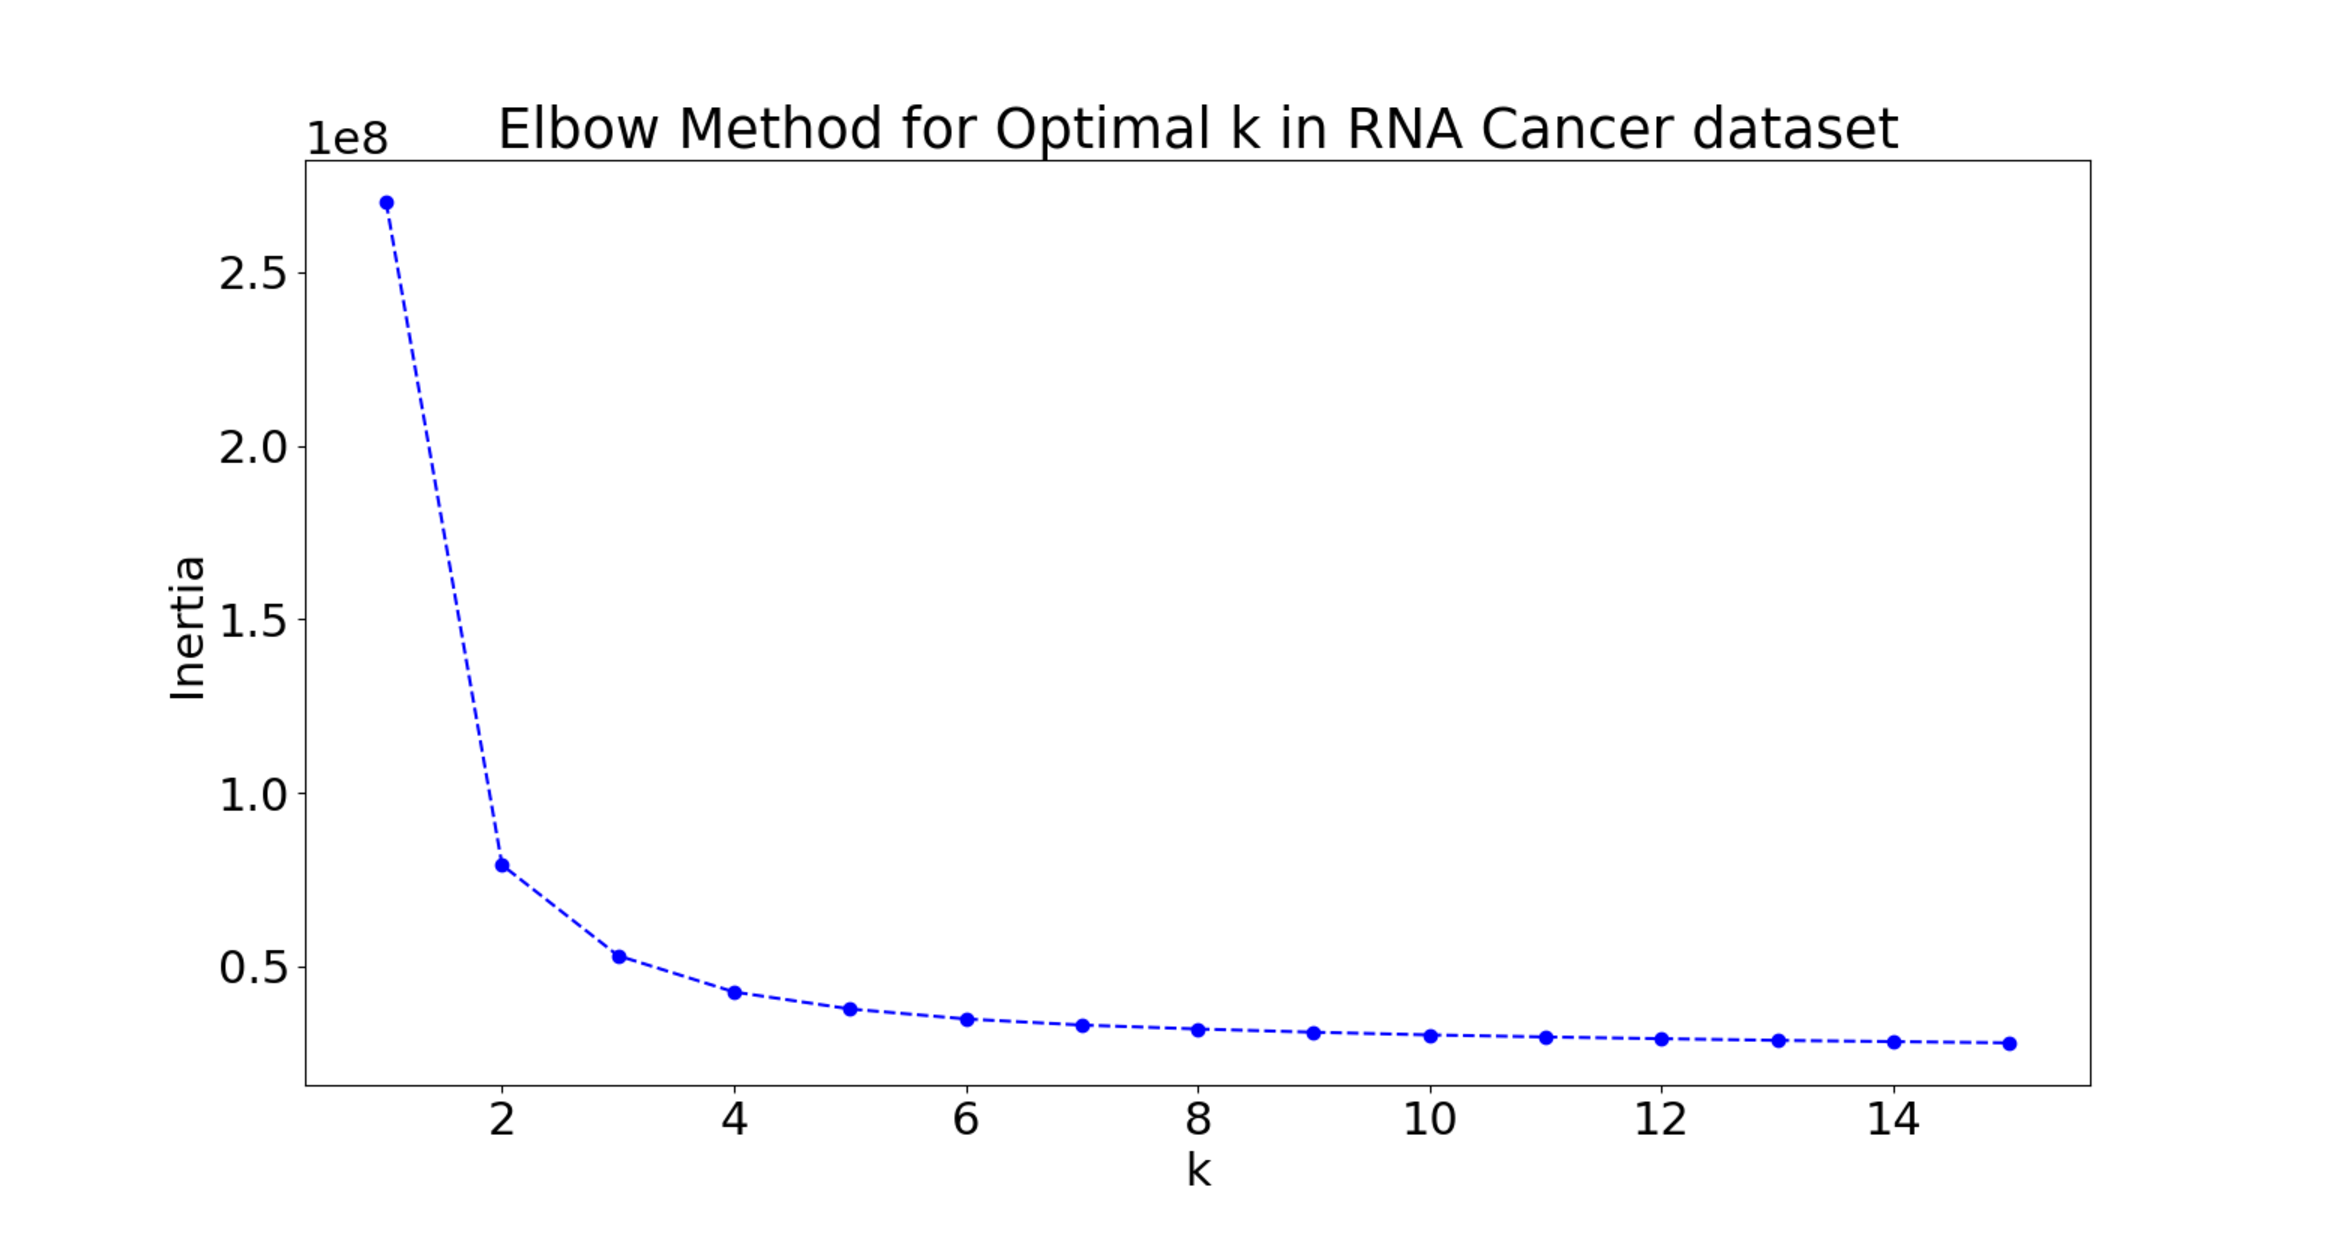
\includegraphics[scale=0.38]{Pictures/cancer_kmeans_800}
		\caption{variation of $k$-means inertia with number of clusters $k$ for RNA dataset}
		\label{fig:kmeans-cancer}
	\end{figure}
\end{center}

\begin{center}
	\begin{figure}[htpb]
		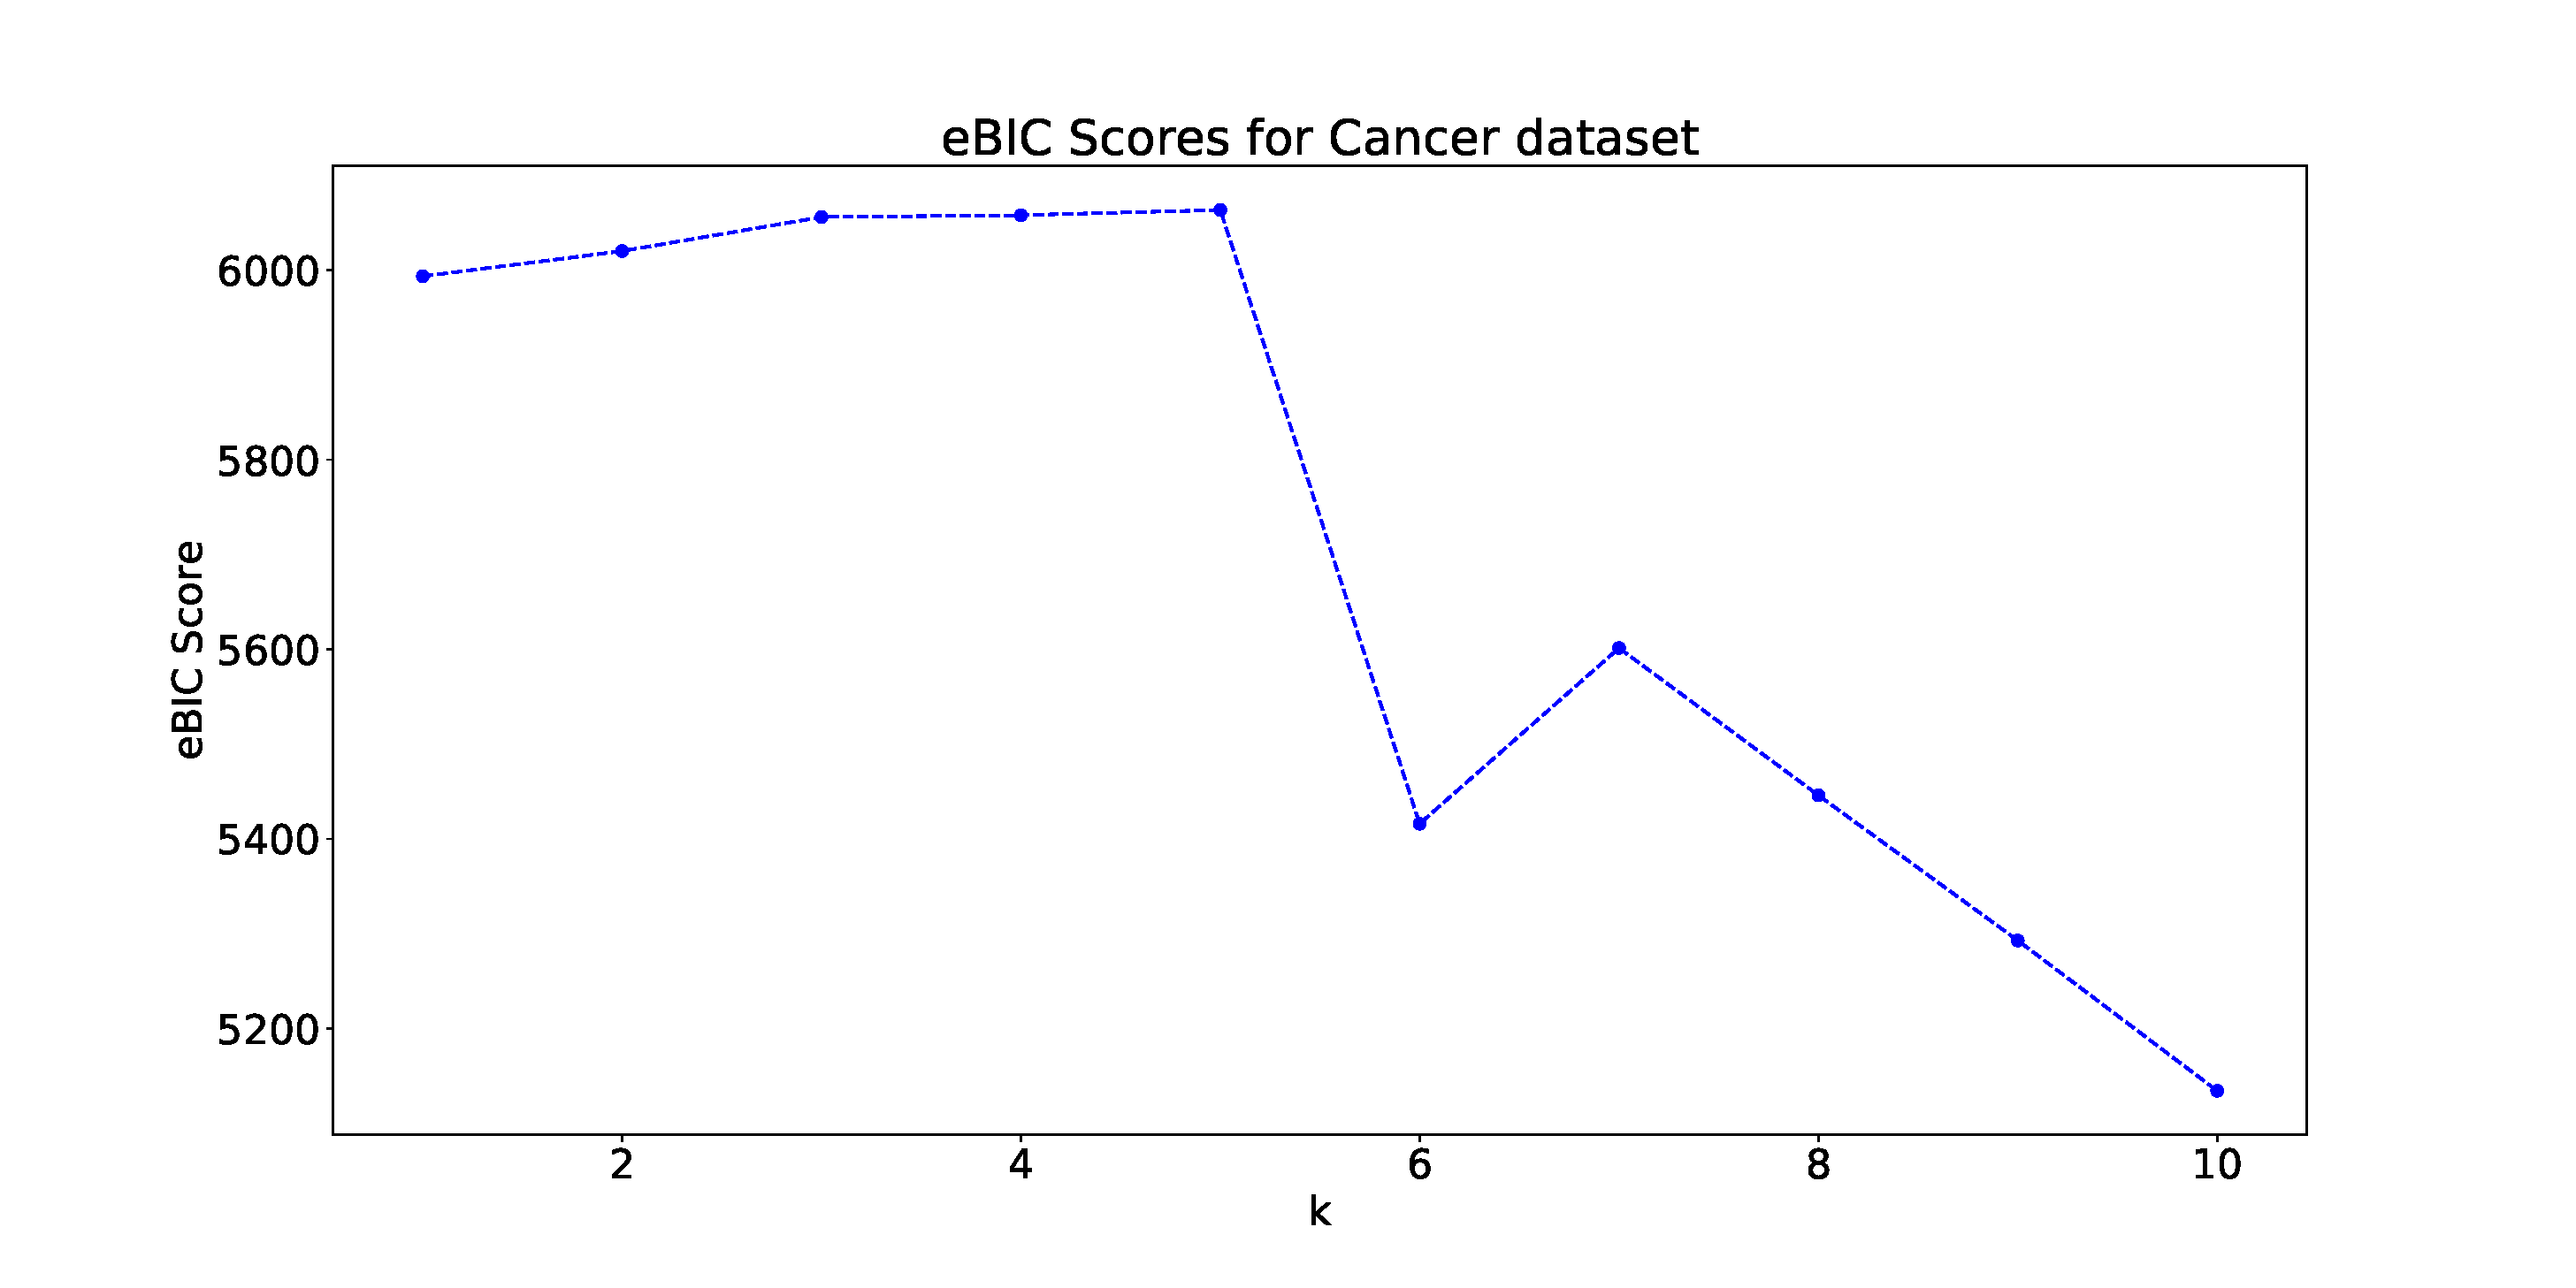
\includegraphics[scale=0.3]{Pictures/cancer}
		\caption{eBIC scores of estimated k-component graphs for RNA dataset}
		\label{fig:gms-cancer}
	\end{figure}
\end{center}

%\subsubsection{Abalone dataset}
%\begin{center}
%	\begin{figure}[htpb]
%		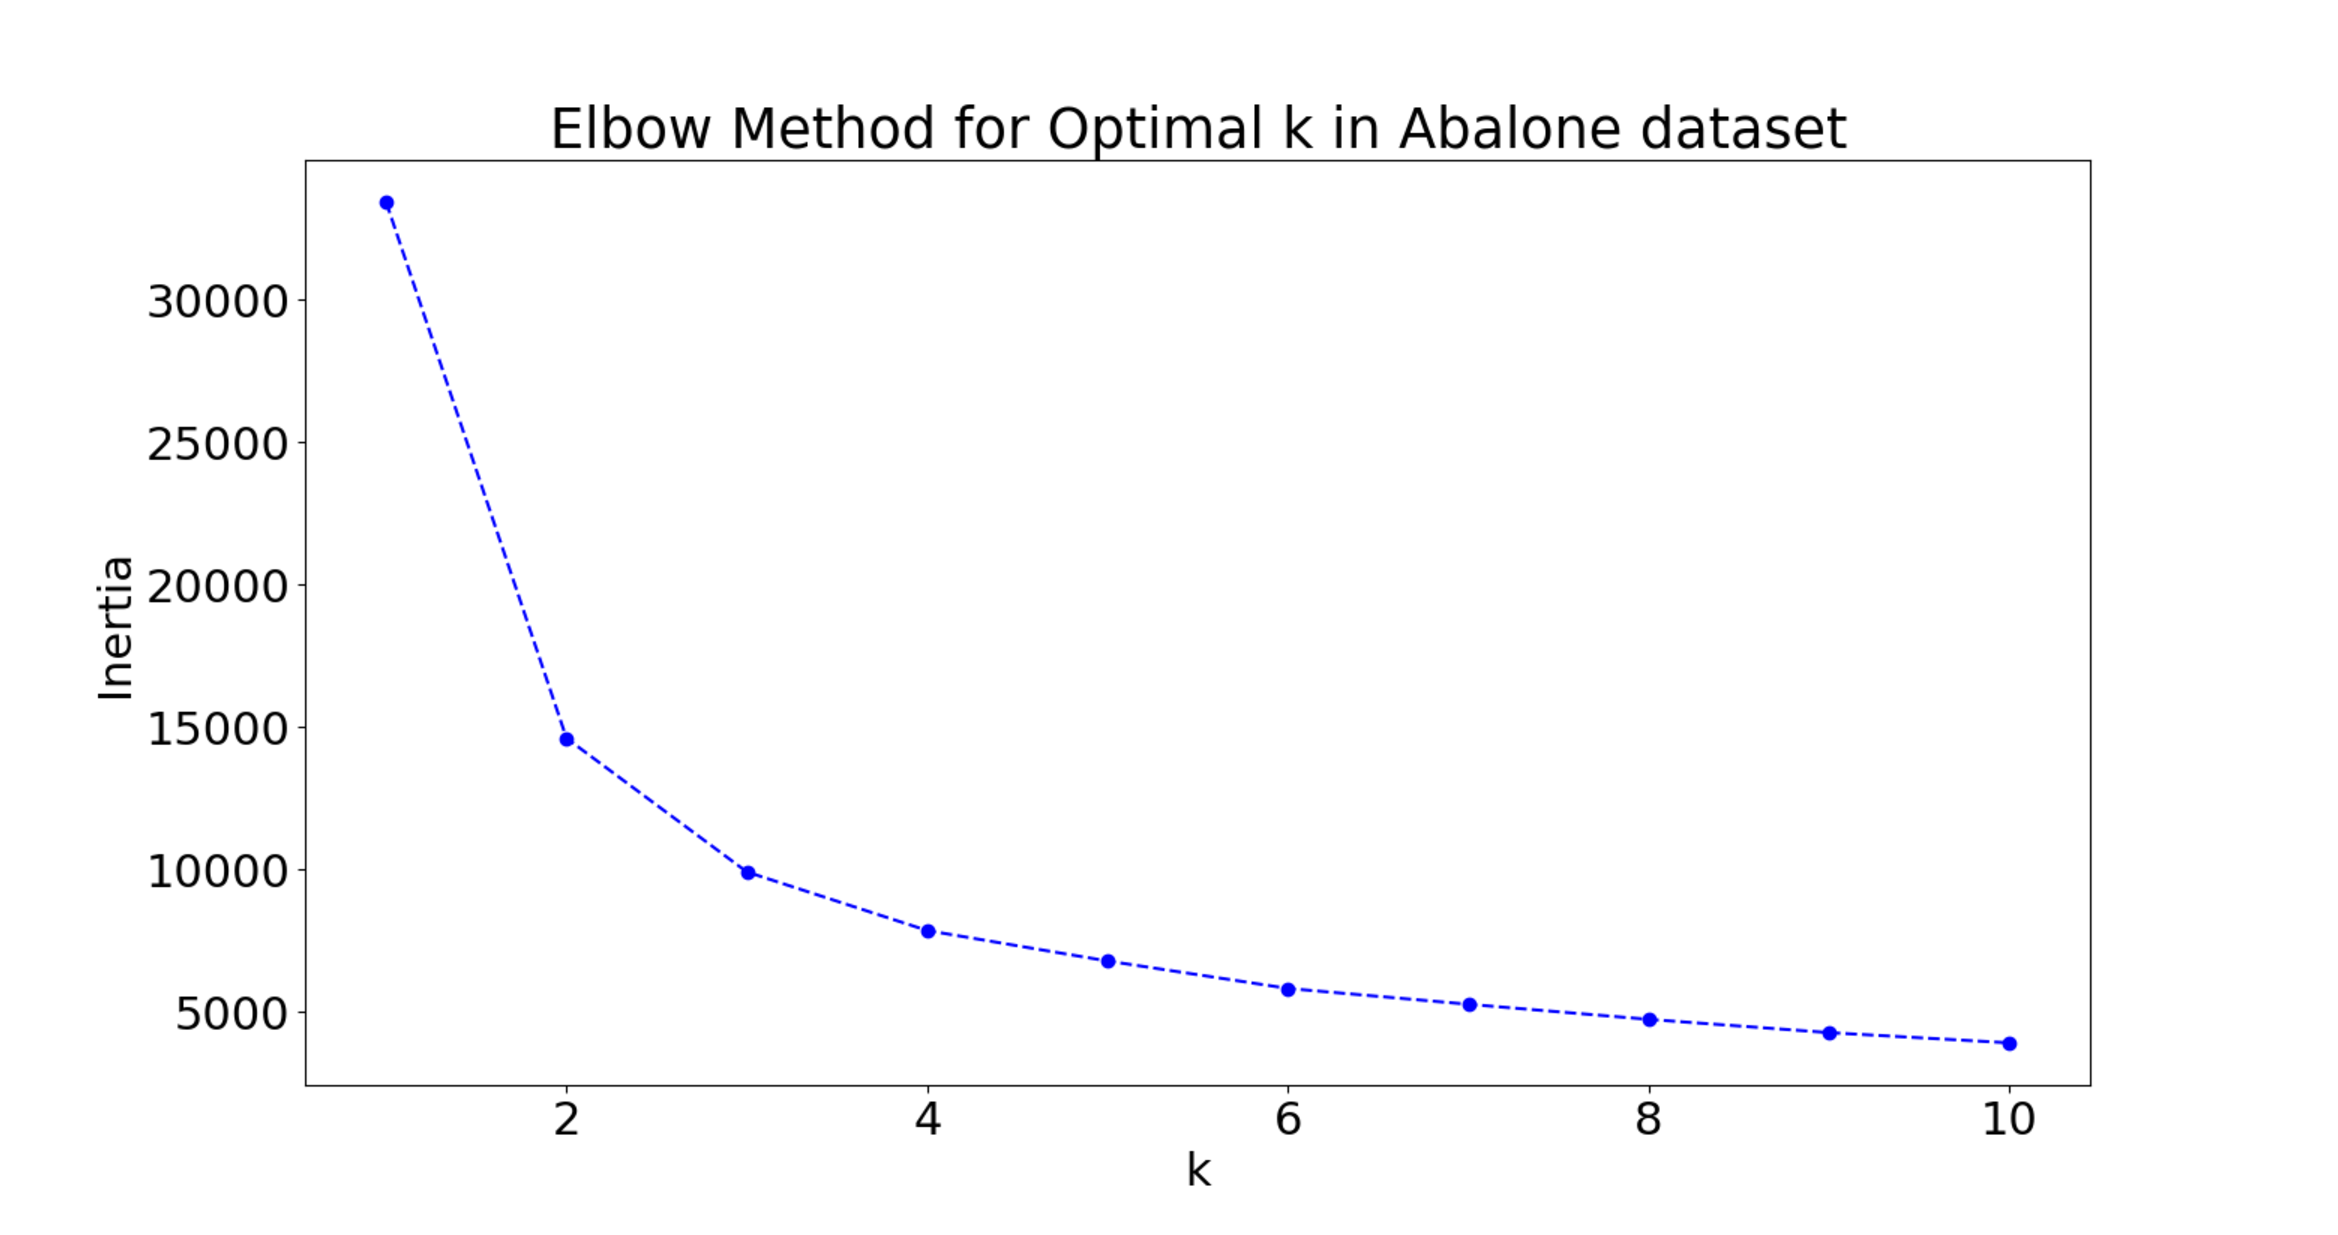
\includegraphics[scale=0.35]{Pictures/abalone_kmeans}
%		\caption{variation of $k$-means inertia with number of clusters $k$ for Abalone dataset}
%		\label{fig:kmeans-abalone}
%	\end{figure}
%\end{center}

%\subsubsection{Yeast dataset}
%\begin{center}
%	\begin{figure}[htpb]
%		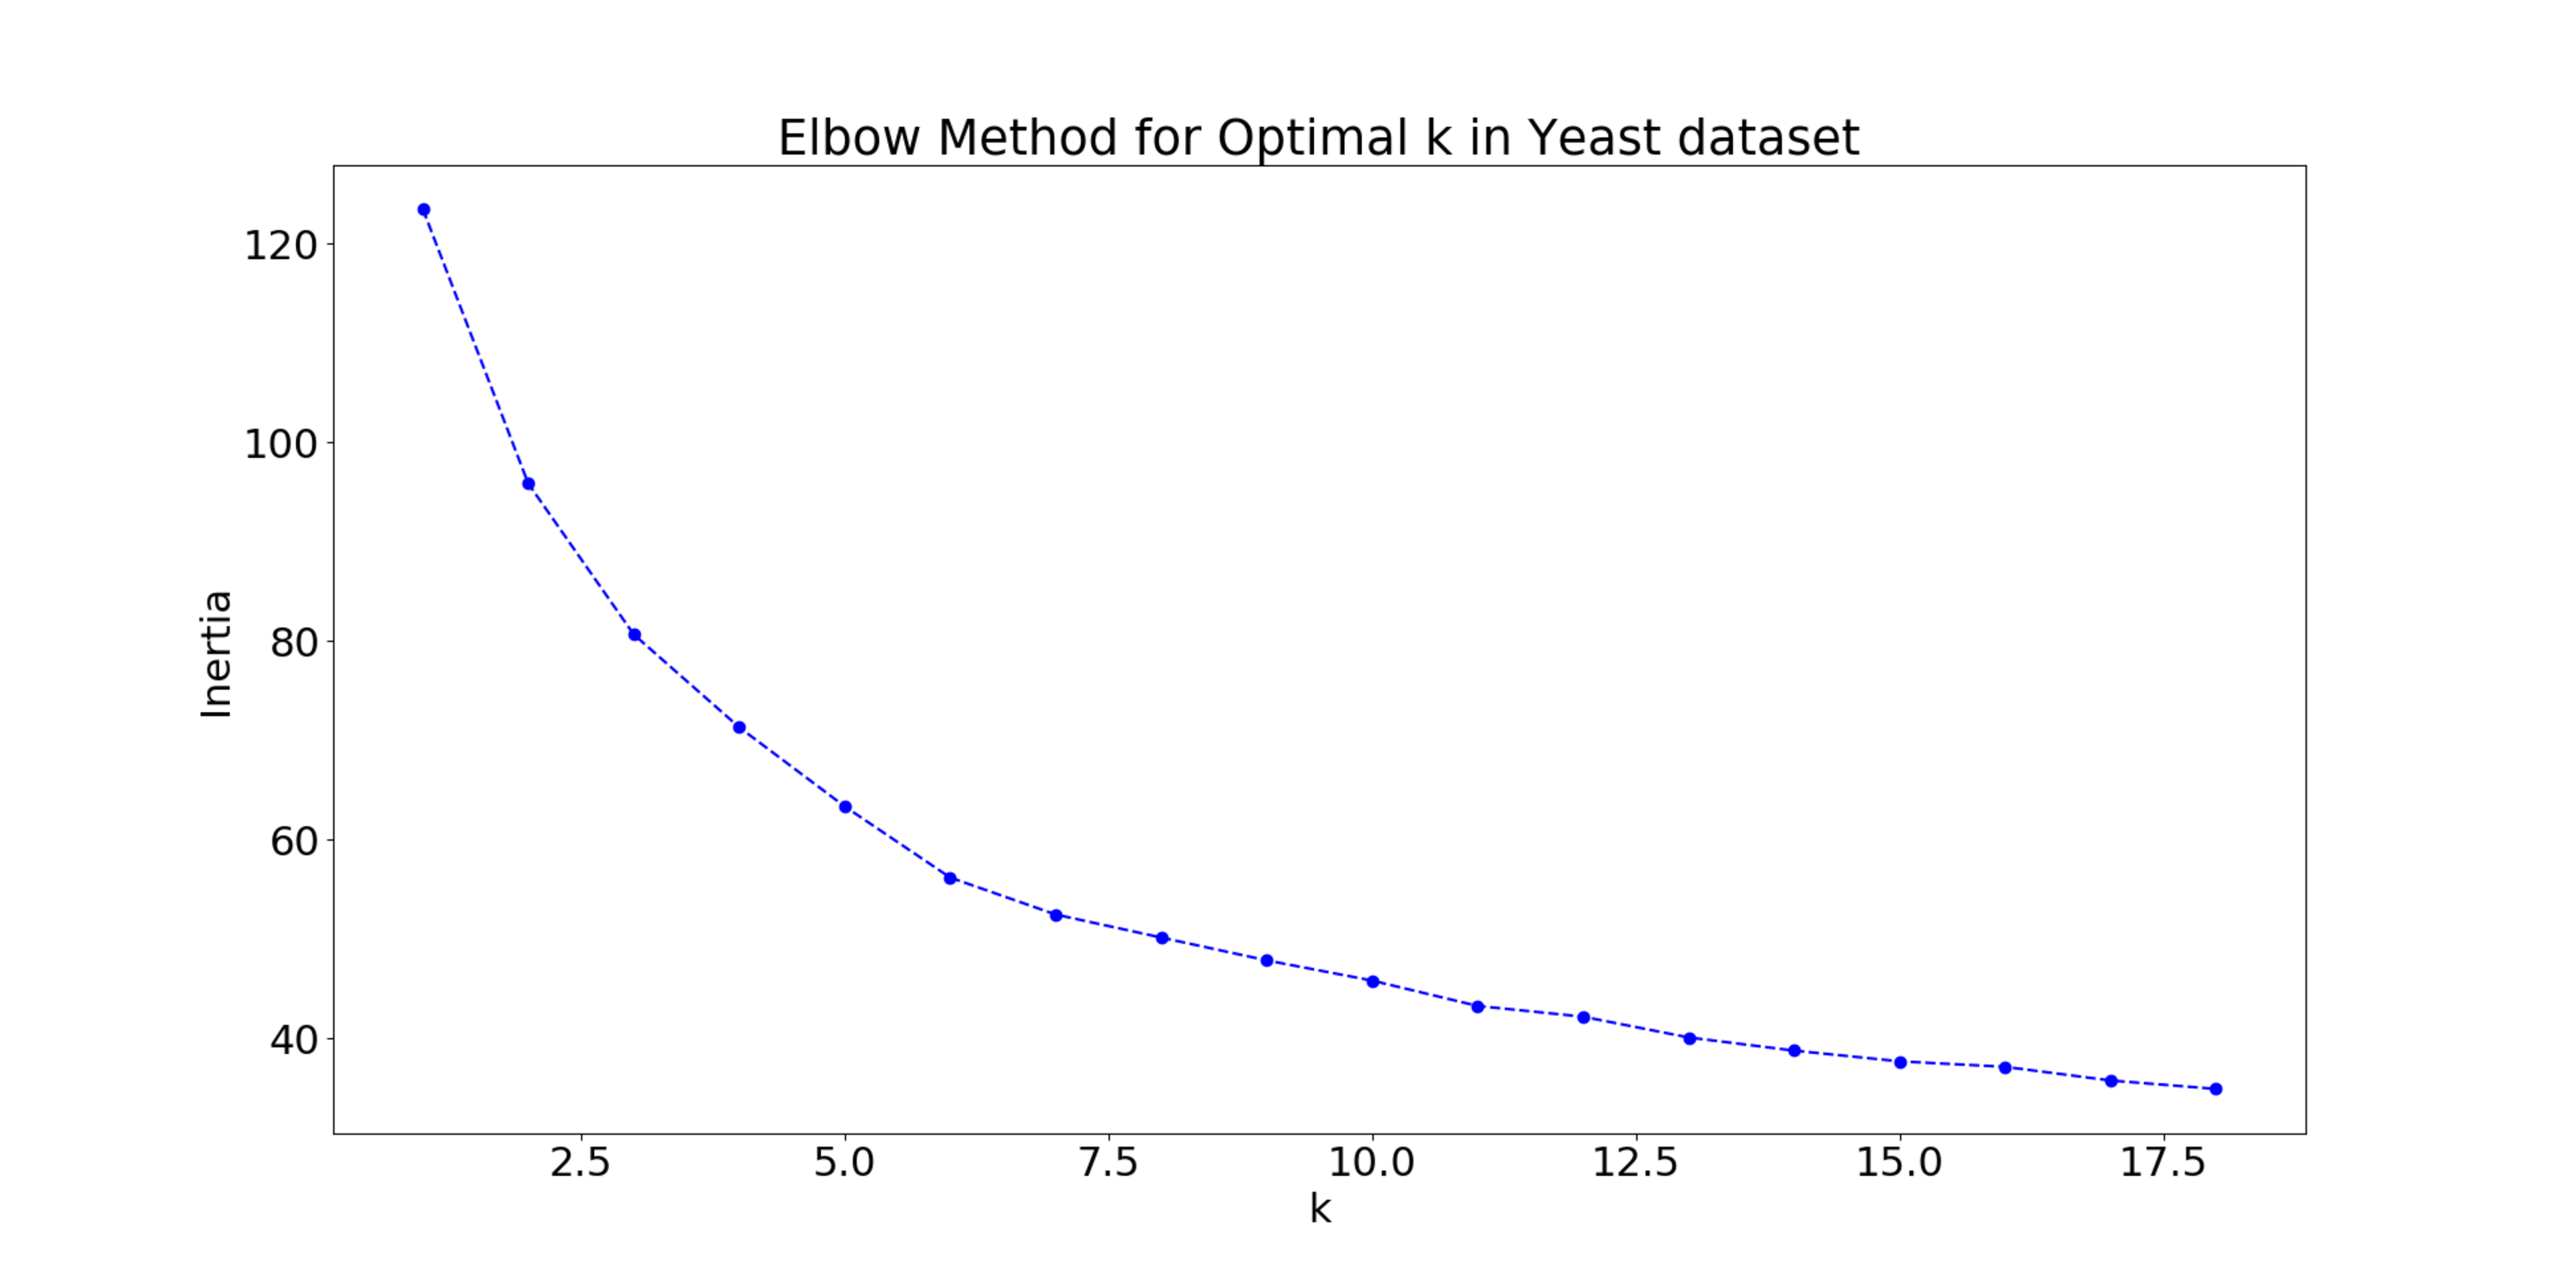
\includegraphics[scale=0.35]{Pictures/yeast_kmeans}
%		\caption{variation of $k$-means inertia with number of clusters $k$ for Yeast dataset}
%		\label{fig:kmeans-yeast}
%	\end{figure}
%\end{center}

\subsubsection{Iris dataset}
The iris dataset has 3 classes corresponding to each species of iris flower. Fig~\ref{fig:kmeans-iris} shows the WSS scores for different values of k indicating that $k=3$ or $k=4$ number of clusters must be there. Fig~\ref{fig:gms-iris} shows the eBIC scores using our proposed component identification algorithm. It can be seen that after $k=3$, eBIC scores fall down indicating that $k=3$ should be the true number of clusters or components in the data. The eBIC scores for $k<3$ are similar to $k=3$. We again attribute this to the model mismatch of SGL algorithm. 
\begin{center}
	\begin{figure}[htpb]
		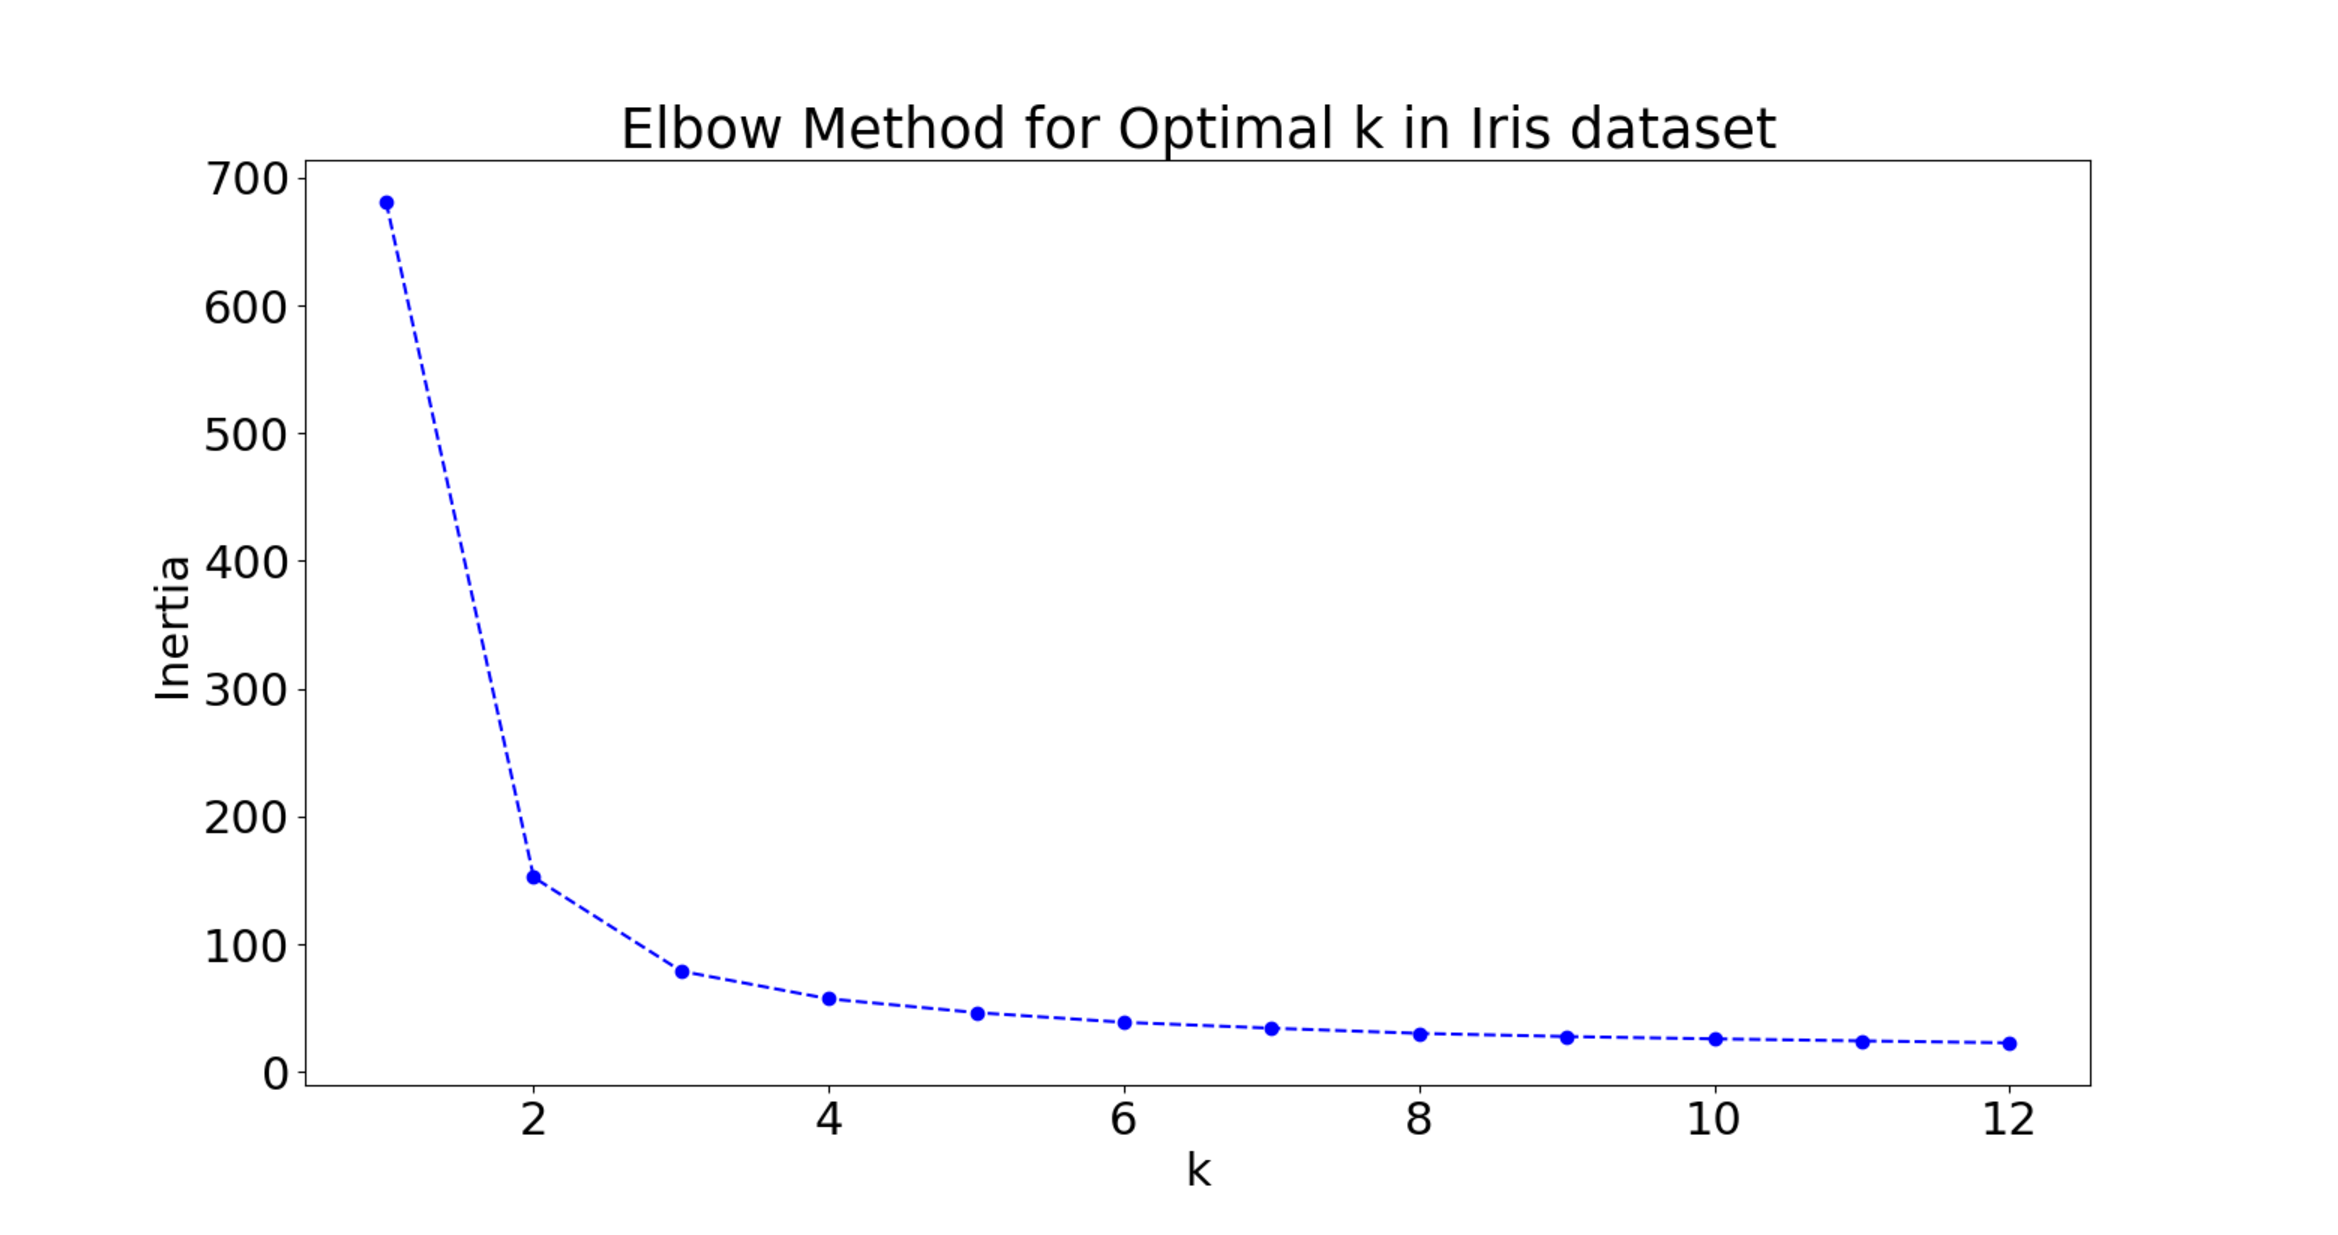
\includegraphics[scale=0.35]{Pictures/iris_kmeans}
		\caption{variation of $k$-means inertia with number of clusters $k$ for Iris dataset}
		\label{fig:kmeans-iris}
	\end{figure}
\end{center}

\begin{center}
	\begin{figure}[htpb]
		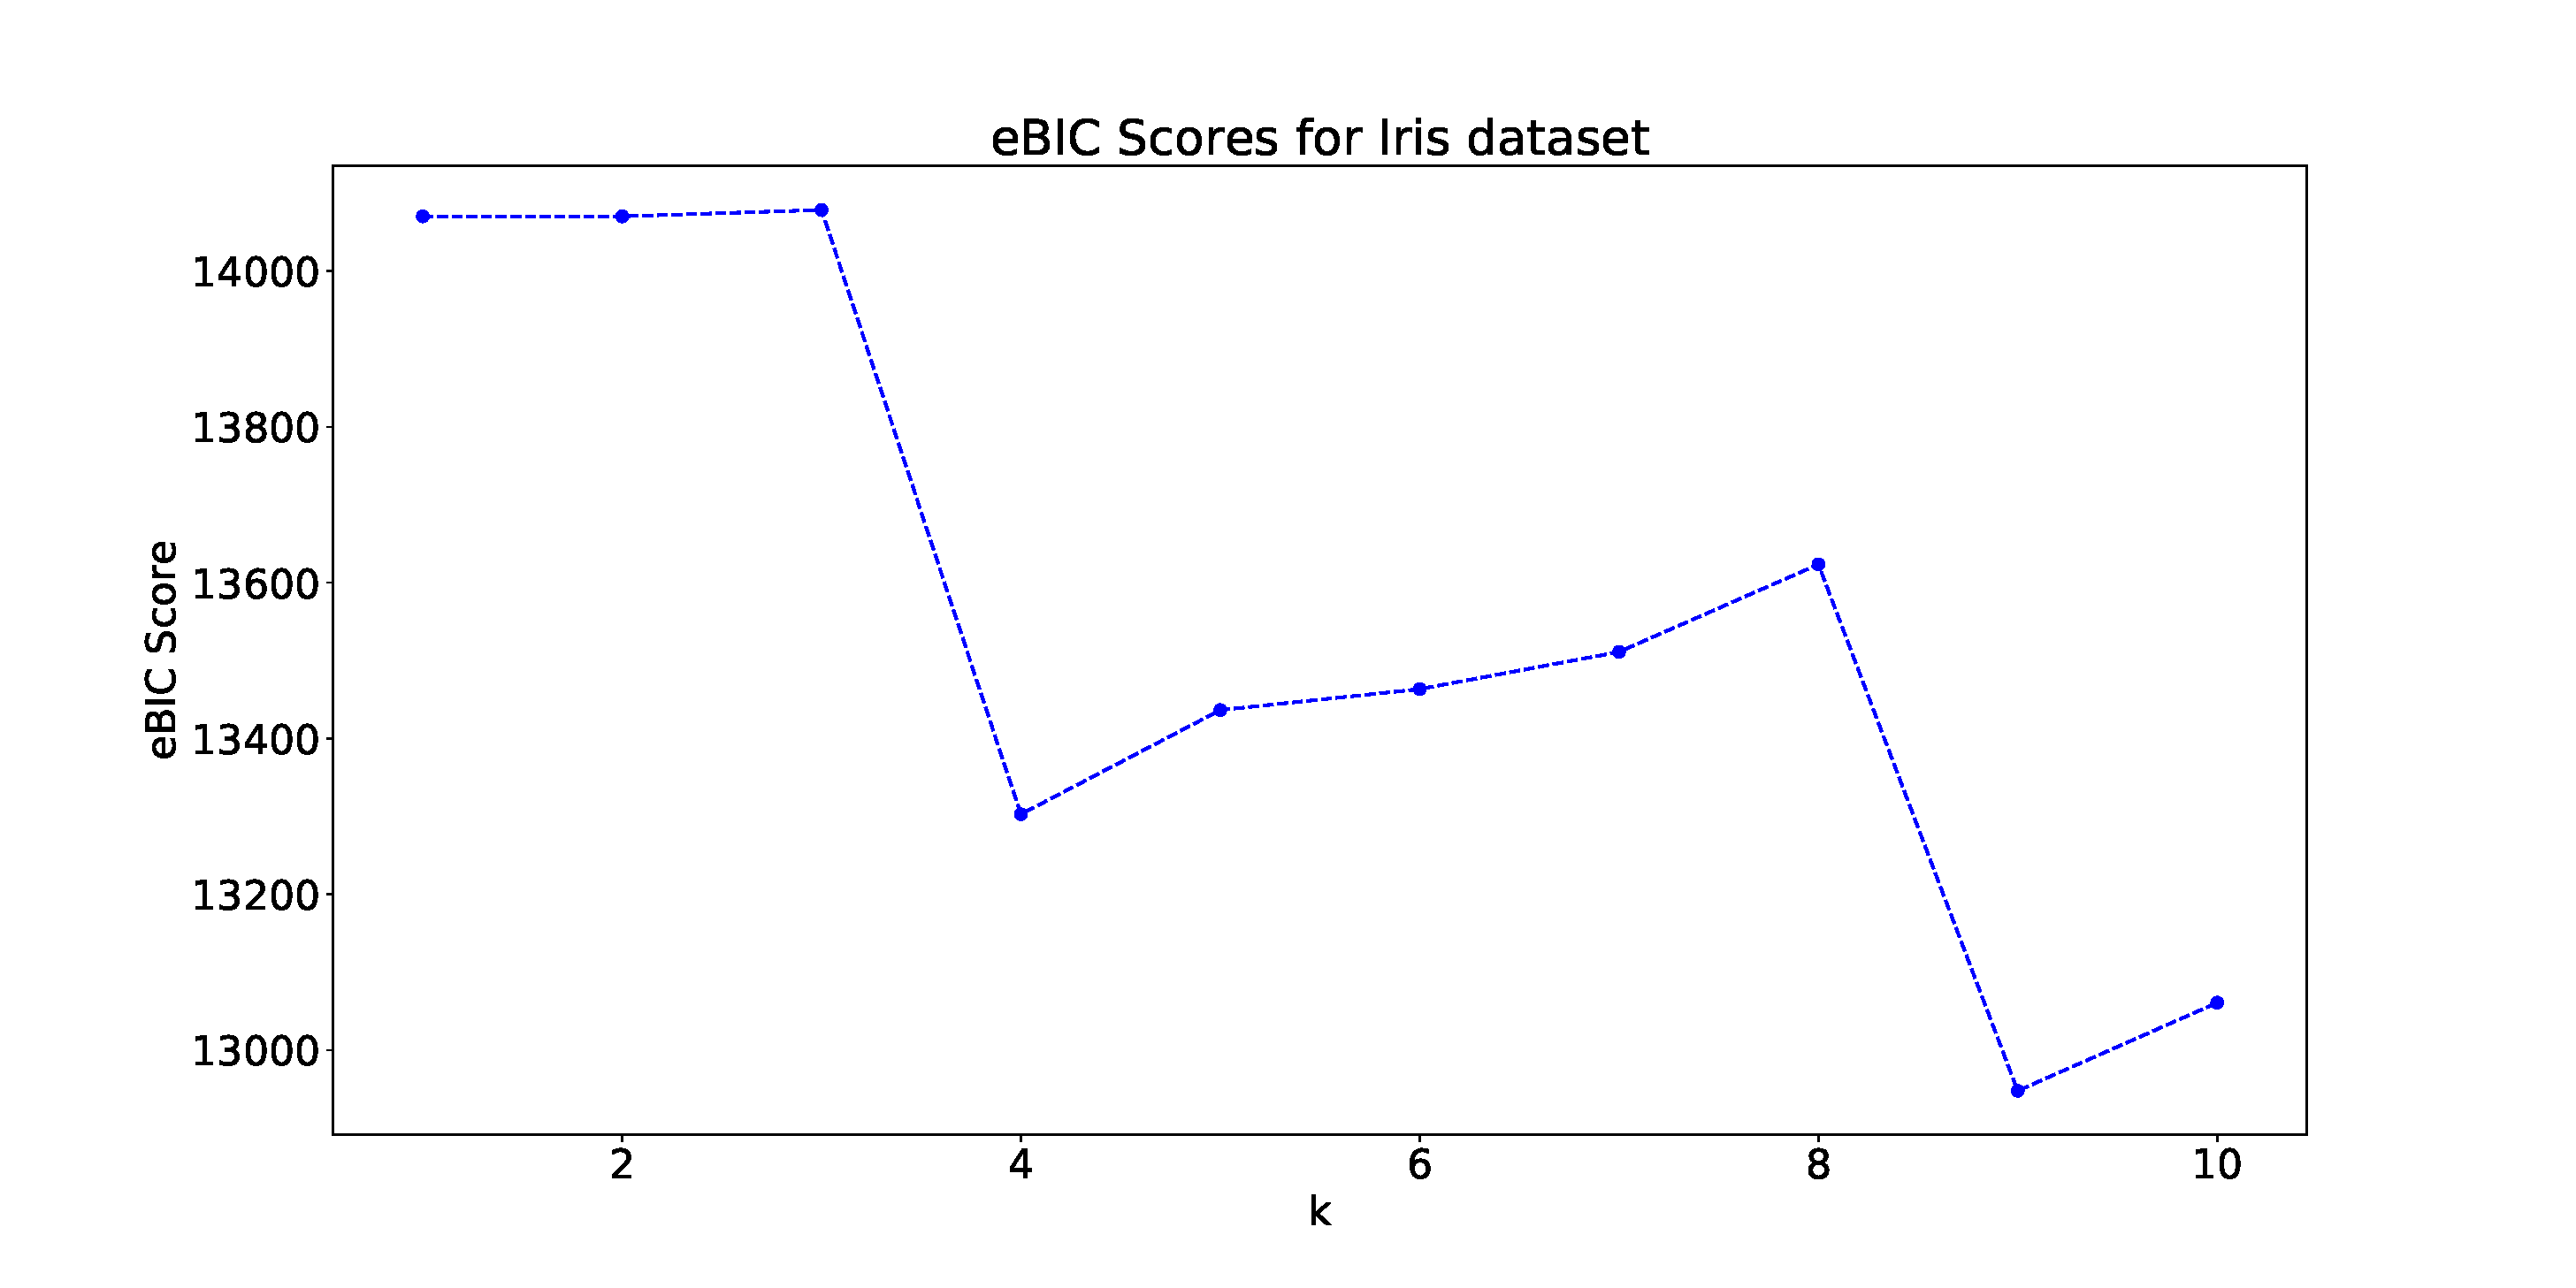
\includegraphics[scale=0.3]{Pictures/iris}
		\caption{eBIC scores of estimated k-component graphs for Iris dataset}
		\label{fig:gms-iris}
	\end{figure}
\end{center}

%\subsubsection{Animals dataset}


\subsection{Bipartite identification}
\subsubsection{Synthetic datasets}
\textbf{Data:} samples $\mathbf{X}=\left\{\mathbf{x}^{(i)} \in \mathbb{R}^{p}\right\}_{i=1}^{n}$ from bipartite GGM with 10 nodes in both sets making $p=20$ and $n=1600$ samples.

Fig~\ref{fig:bip-adj} shows the true, empirical and learned adjacency matrix using 1-component SGL and SGA algorithm respectively. Both the SGL and SGA algorithms are only provided with the sample covariance matrix $S$. It can be visually confirmed that SGA has learned graph which is more likely to be the true graph. We compute eBIC scores (higher is better) for the two graph structures in Table~\ref{tab:bip-res}. It is evident that our proposed Algorithm~\ref{alg:bip-id} selects the bipartite structure, which is indeed the underlying graph structure in this case. This upholds the validity of our proposed algorithm.

\begin{figure}[htpb]
	\begin{center}
		\resizebox{50mm}{!} {\includegraphics *{bipartite_true_adj.eps}}
		\resizebox{50mm}{!} {\includegraphics *{bipartite_estimated_adj_empirical.eps}}
		\resizebox{50mm}{!} {\includegraphics *{bipartite_1comp_estimated_adj.eps}}
		\resizebox{50mm}{!} {\includegraphics *{bipartite_estimated_adj.eps}}
		
		\caption {First row: True Adjacency matrix for bipartite GGM; empirical adjacency matrix respectively. Second row: adjacency matrix learned using 1-component SGL algorithm; adjacency matrix learned using bipartite SGA algorithm.}
		\label{fig:bip-adj}
	\end{center}
\end{figure}

\begin{table}[htpb]
	\caption{Bipartite identification results on bipartite GGM with 10 nodes in both set}
	\label{tab:bip-res}
	\centering
	\begin{tabular}{llll}
		\toprule
		Metric     &   F1-Score  & Relative Error & eBIC Score \\
		\midrule
		True Adj          & 1.0    & 0     &       \\
		Empirical Adj     & 0.689  & 0.123 &        \\
		1-component Adj   & 0.766  & 0.997 & $-512.066$   \\
		Bipartite Adj     & 0.959  & 0.134 & $-176.895$  \\
		\bottomrule
	\end{tabular}
\end{table}

\textbf{Data:} samples $\mathbf{X}=\left\{\mathbf{x}^{(i)} \in \mathbb{R}^{p}\right\}_{i=1}^{n}$ from bipartite GGM with 10 and 6 nodes in each set making $p=16$ and $n=1600$ samples. 

Given a data sampled from bipartite GGM, our algorithm always selects bipartite structure in contrast to the $k$-component structure. We have confirmed this observation with different numbers of nodes in each sets and different number of samples. Table~\ref{tab:bip-res2} shows results for the above data, validating the algorithm. Though the scalability of nodes couldn't be tested due to $O(p^3)$ complexity of the algorithm.

\begin{table}[htpb]
	\caption{Bipartite identification results on bipartite GGM with 10 and 6 nodes in each set}
	\label{tab:bip-res2}
	\centering
	\begin{tabular}{llll}
		\toprule
		Metric     &   F1-Score  & Relative Error & eBIC Score \\
		\midrule
		True Adj          & 1.0    & 0     &        \\
		Empirical Adj     & 0.667  & 0.117 &        \\
		1-component Adj   & 0.708  & 0.122 & $-458.748$   \\
		Bipartite Adj     & 0.957  & 0.158 & $-198.36$  \\
		\bottomrule
	\end{tabular}
\end{table}